\documentclass{article}
\usepackage{amsmath}
\usepackage{mathtools}
\usepackage{gensymb}
\usepackage[a4paper,inner=1.5cm,outer=1.5cm,top=2cm,bottom=0.5cm]{geometry} 
\usepackage{xcolor}                    
\usepackage{tikz}                           
\usepackage{multicol}
\usepackage{pgfplots}
\usetikzlibrary{calc}
\usetikzlibrary{intersections}
\usetikzlibrary{intersections,calc,angles,quotes}
\usetikzlibrary{shapes,arrows,positioning,decorations.pathreplacing,calc}
\usetikzlibrary{calc,angles,positioning,intersections,quotes,decorations.markings}
\usepackage{tkz-euclide}
\usetikzlibrary{backgrounds}
\usetikzlibrary{calc,through}
\usetikzlibrary{angles}
\usetikzlibrary{fadings}
\usetikzlibrary{shapes.geometric}
\usetikzlibrary{shapes.symbols}
\usepackage{draftwatermark}
\usepackage{mathptmx}

\SetWatermarkText{\textcolor{black!20}{Mathema Shukur}}
\SetWatermarkFontSize{2 cm}
\usepackage[utf8]{inputenc}
\usepackage{fontspec}

\setmainfont{[Kalpurush.ttf]}
\newfontface{\en}{[Arial.ttf]} %%this is optional, if you want to use a secondary font. Any english font is supported
\newlength\Radius
\setlength\Radius{4cm}
\begin{document} 
	\Large
	\textcolor{red}{Welcome To} 
	\\
	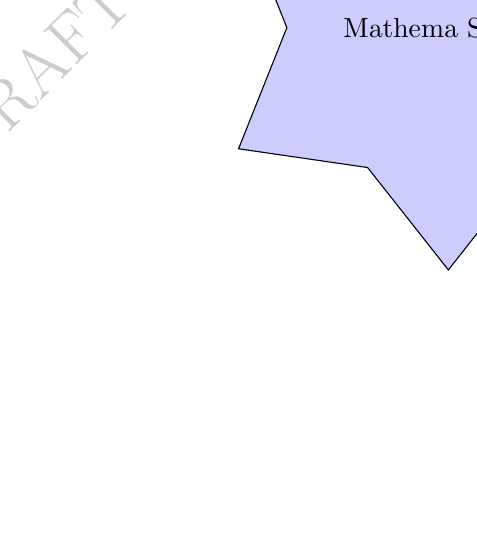
\begin{tikzpicture}
		\tikz \node [fill=blue!20,star,star points=6,draw] {Mathema Shukur };
	\end{tikzpicture}
	\\
	যাদের জন্যে প্রযোজ্যঃ  	\textcolor{magenta}{একাদশ ও দ্বাদশ শ্রেণীর শিক্ষার্থী} \\
	বিষয়ঃ \textcolor{magenta}{উচ্চতর গণিত ১ম পত্র} \\
	অধ্যায়ঃ \textcolor{magenta}{৪-বৃত্ত}\\ 
	\\
	\\
	(১)  মূল বিন্দুতে কেন্দ্র বিশিষ্ট বৃত্তের সমীকরণ  \\
	\\
	\textcolor{blue}{$x^2+y^2=r^2$}\\
	\\
	(২) নির্দিষ্ট কেন্দ্র ও ব্যাসার্ধ বিশিষ্ট বৃত্তের  সমীকরণ \\
	\\
	\textcolor{blue}{$(x-h)^2+(y-k)^2=r^2$}\\
	\\
	(৩) বৃত্তের সাধারণ সমীকরণ\\
	\\  
	\textcolor{blue}{$x^2+y^2+2gx+2fy+c=0$}\\
	\\
	(৪) ব্যাসের প্রান্ত বিন্দুদ্বয় $(x_1,y_1)$ এবং $(x_2,y_2)$ হলে বৃত্তের সমীকরণ\\
	\\ 
	\textcolor{blue}{$(x-x_1)(x-x_2)+(y-y_1)(y-y_2)=0$}\\
	\\
	(৫) একটি বৃত্ত \textcolor{blue}{$S=0$ }এবং একটি সরলরেখা \textcolor{blue}{$L=0$}  এর ছেদবিন্দুগামী বৃত্তের সমীকরণ  \textcolor{blue}{$S+kL=0$} \\
	\\
	(৬) দুইটি বৃত্ত \textcolor{blue}{$S_1=0$} ও \textcolor{blue}{$S_2=0$} এর ছেদবিন্দুগামী বৃত্তের সমীকরণ \textcolor{blue}{$S_1+kS_2=0$}\\  \\
	(৭) পোলার স্থানাঙ্কে বৃত্তের  সমীকরণ \\
	\textcolor{blue}{$r^2+2r(g\cos \theta+f\sin \theta )+c=0$}\\
যেখানে 	$g=-\rho \cos \alpha,\,\,\,f=-\rho \sin \alpha,\,\,\,c=\rho^2-a^2 $\\
	\\ 
	$(x_1,y_1)$ ও $(x_2,y_2)$ বিন্দু দুইটির সংযোগ রেখাংশকে ব্যাস ধরে অঙ্কিত বৃত্তের সমীকরণ \\
	\\ 
	$\textcolor{blue}{(x-x_1)(x-x_2)+(y-y_1)(y-y_2)=0}$\\
	\\
		\begin{tikzpicture}[transform shape,scale=1]
		\draw [-latex,thick,red](-2,0) -- (10,0) node[right] {$x$} coordinate(x axis);
		\draw [-latex,thick,red](0,-2) -- (0,10) node[above] {$y$} coordinate(y axis);
		\fill[black] (0,0) circle (1 mm);
		\node at (0.8,-0.3) {$\textcolor{red}{O(0,0)}$};	
		\draw[thick,blue] (5,5) circle (3);
		\fill[blue] (5,5) circle (1 mm);
		\node at (5,8.5) {$\textcolor{blue}{C(x,y)}$};
			\fill[blue] (5,8) circle (1 mm);
		\node at (1,5) {$\textcolor{blue}{A(x_1,y_1)}$};
		\fill[blue] (2,5) circle (1 mm);
		\node at (9,5) {$\textcolor{blue}{B(x_2,y_2)}$};
		\fill[blue] (8,5) circle (1 mm);
		\draw[red,dashed] (2,5)--(8,5);
	\end{tikzpicture}\\
\\
		\textcolor{blue}{[ঢাকা বিশ্ববিদ্যালয় ভর্তি পরীক্ষা -২০১৫-২০১৬]}\\
	$(-4,3)$ এবং  $(12,-1)$ বিন্দুদ্বয়ের সংযোগ রেখাংশকে ব্যাস ধরে অঙ্কিত বৃত্তের সমীকরণ নির্ণয় কর । \\
	$(x_1,y_1)=(-4,3)$;\hspace{2cm} $(x_2,y_2)=(12,-1)$\\
	\begin{align*}
		(x-x_1)(x-x_2)+(y-y_1)(y-y_2)&=0\\
		\\
		(x-(-4))(x-12)+(y-3)(y-(-1))&=0\\
		\\
		(x+4)(x-12)+(y-3)(y+1)&=0\\
		\\
		x^2-12x+4x-48+y^2+y-3y-3&=0\\
		\\
		x^2+y^2-8x-2y-51&=0
	\end{align*}
	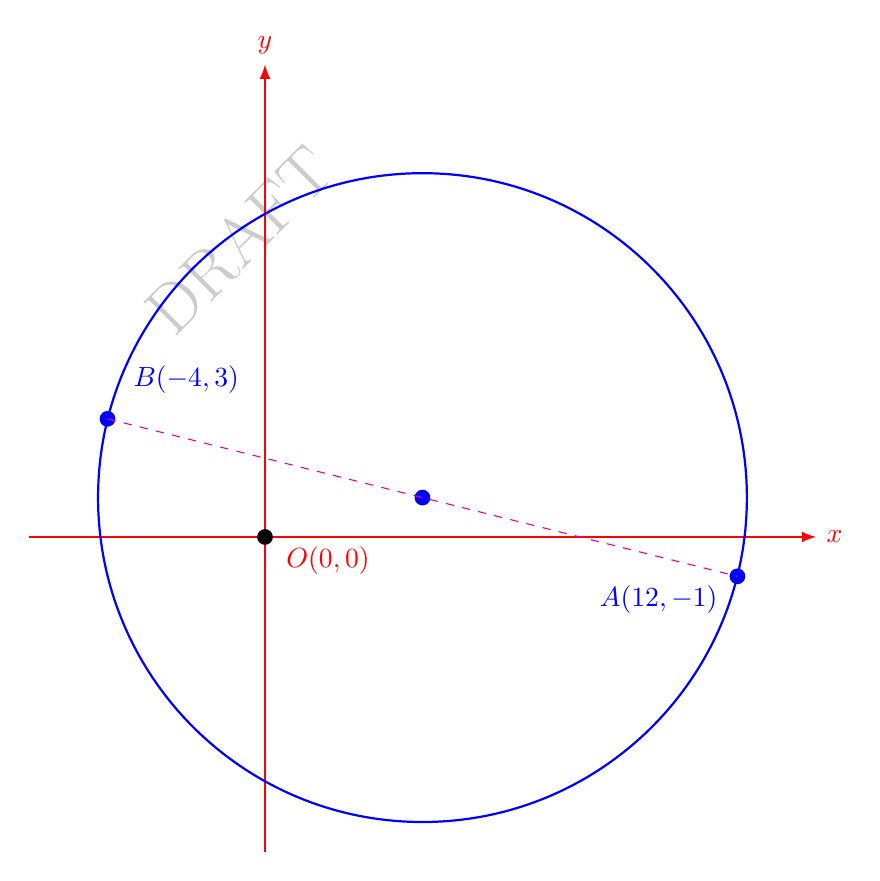
\begin{tikzpicture}[transform shape,scale=1]
		\draw [-latex,thick,red](-3,0) -- (7,0) node[right] {$x$} coordinate(x axis);
		\draw [-latex,thick,red](0,-4) -- (0,6) node[above] {$y$} coordinate(y axis);
		\fill[black] (0,0) circle (1 mm);
		\node at (0.8,-0.3) {$\textcolor{red}{O(0,0)}$};	
		\draw[thick,blue] (2,0.5) circle (4.12);
		\fill[blue] (2,0.5) circle (1 mm);
		\fill[blue] (-2,1.5 ) circle (1 mm);
		\fill[blue] (6,-0.5) circle (1 mm);
		\node at (5,-0.8) {$\textcolor{blue}{A(12,-1)}$};
		\node at (-1,2) {$\textcolor{blue}{B(-4,3)}$};
		\draw[magenta,dashed](-2,1.5)--(6,-0.5);
	\end{tikzpicture}\\
		\textcolor{blue}{[ঢাকা বিশ্ববিদ্যালয় ভর্তি পরীক্ষা -২০১৭-২০১৮]}\\
 মূলবিন্দুগামী একটি বৃত্ত ধনাত্মক $x-$ অক্ষ হতে $4$ একক এবং ধনাত্মক  $y-$ অক্ষ হতে  $2$ একক ছেদক কর্তন করলে এর সমীকরণ নির্ণয় কর। \\ 
	\\
	$(x_1,y_1)=(4,0)$;\hspace{2cm} $(x_2,y_2)=(0,2)$\\
	\begin{align*}
		(x-x_1)(x-x_2)+(y-y_1)(y-y_2)&=0\\
		\\
		(x-4)(x-0)+(y-0)(y-2)&=0\\
		\\
		x^2-4x+y^2-2y&=0\\
		\\
		x^2+y^2-4x-2y&=0\\
	\end{align*}
		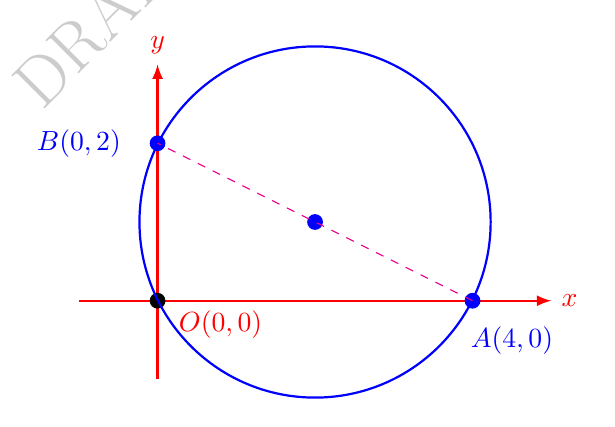
\begin{tikzpicture}[transform shape,scale=1]
		\draw [-latex,thick,red](-1,0) -- (5,0) node[right] {$x$} coordinate(x axis);
		\draw [-latex,thick,red](0,-1) -- (0,3) node[above] {$y$} coordinate(y axis);
		\fill[black] (0,0) circle (1 mm);
		\node at (0.8,-0.3) {$\textcolor{red}{O(0,0)}$};	
		\draw[thick,blue] (2,1) circle (2.23);
		\fill[blue] (2,1 ) circle (1 mm);
		\fill[blue] (4,0) circle (1 mm);
		\node at (4.5,-0.5) {$\textcolor{blue}{A(4,0)}$};
		\fill[blue] (0,2) circle (1 mm);
		\node at (-1,2) {$\textcolor{blue}{B(0,2)}$};
		\draw[magenta,dashed](4,0)--(0,2);
	\end{tikzpicture}\\
	\\
	\\
	\\
		\textcolor{blue}{[BUET-2010-2011]}\\
	$(0,-1)$ এবং  $(2,3)$ বিন্দুদ্বয়ের সংযোগ রেখাকে ব্যাস ধরে অঙ্কিত বৃত্তটি $x-$ অক্ষের থেকে যে পরিমান অংশ ছেদ করে তা নির্ণয় কর।  । \\
	\\
	$(x_1,y_1)=(0,-1)$;\hspace{2cm} $(x_2,y_2)=(2,3)$\\
	\\
	\begin{align*}
		(x-x_1)(x-x_2)+(y-y_1)(y-y_2)&=0\\
		\\
		(x-0)(x-2)+(y-(-1))(y-3)&=0\\
		\\
		x^2-2x+(y-3)(y+1)&=0\\
		\\
		x^2-2x+y^2+y-3y-3&=0\\
		\\
		x^2+y^2-2x-2y-3&=0\\
		\\
		x^2+y^2+2(-1)x+2(-1)y+(-3)&=0\\
		\\
		g=-1,\,\,\,f=-1,&\,\,\,c=-3
	\end{align*}
$x-$ অক্ষের খন্ডিত অংশের দৈর্ঘ্য  $2\sqrt{g^2-c}=2\sqrt{(-1)^2-(-3)}=2\sqrt{10}$\\
		\begin{tikzpicture}[transform shape,scale=1]
		\draw [-latex,thick,red](-3,0) -- (7,0) node[right] {$x$} coordinate(x axis);
		\draw [-latex,thick,red](0,-4) -- (0,6) node[above] {$y$} coordinate(y axis);
		\fill[black] (0,0) circle (1 mm);
		\node at (0.8,-0.3) {$\textcolor{red}{O(0,0)}$};	
		\draw[thick,blue] (1,1) circle (2.23);
		\fill[blue] (1,1) circle (1 mm);
		\fill[blue] (0,-1 ) circle (1 mm);
		\fill[blue] (2,3) circle (1 mm);
		\node at (1,-1.5) {$\textcolor{blue}{A(0,-1)}$};
		\node at (2,3.5) {$\textcolor{blue}{B(2,3)}$};
		\draw[magenta,dashed](0,-1)--(2,3);
	\end{tikzpicture}\\
	\\ 
		\textcolor{blue}{[ঢাকা বোর্ড-২০২২]}\\
	$(5,3)$ এবং  $(-5,7)$ বিন্দুদ্বয়ের সংযোগ রেখাংশকে ব্যাস ধরে অঙ্কিত বৃত্তের সমীকরণ নির্ণয় কর । \\
	\\
	$(x_1,y_1)=(5,3)$;\hspace{2cm} $(x_2,y_2)=(-5,7)$\\
	\\
	\begin{align*}
		(x-x_1)(x-x_2)+(y-y_1)(y-y_2)&=0\\
		\\
		(x-5)(x+5)+(y-3)(y-7)&=0\\
		\\
		x^2-25+y^2-10y+21&=0\\
		\\
		x^2+y^2-10y-4&=0
	\end{align*}
		\begin{tikzpicture}[transform shape,scale=1]
		\draw [-latex,thick,red](-7,0) -- (7,0) node[right] {$x$} coordinate(x axis);
		\draw [-latex,thick,red](0,-1) -- (0,11) node[above] {$y$} coordinate(y axis);
		\fill[black] (0,0) circle (1 mm);
		\node at (0.8,-0.3) {$\textcolor{red}{O(0,0)}$};	
		\draw[thick,blue] (0,5) circle (5.38);
		\fill[blue] (0,5) circle (1 mm);
		\fill[blue] (5,3 ) circle (1 mm);
		\fill[blue] (-5,7) circle (1 mm);
		\node at (6,2.5) {$\textcolor{blue}{A(5,3)}$};
		\node at (-4,7) {$\textcolor{blue}{B(-5,7)}$};
		\draw[magenta,dashed](5,3)--(-5,7);
	\end{tikzpicture}\\
	\\ 
		\textcolor{blue}{[চট্রগ্রাম বোর্ড-২০২২]}\\
	$P(2,1)$ এবং  $Q(-6,5)$ বিন্দুদ্বয়ের সংযোগ রেখাংশকে ব্যাস ধরে অঙ্কিত বৃত্তের সমীকরণ নির্ণয় কর ।বৃত্তটি অক্ষদ্বয়ের খন্ডিতাংশের দৈর্ঘ্য নির্ণয় কর।  \\
	\\
	$(x_1,y_1)=(2,1)$;\hspace{2cm} $(x_2,y_2)=(-6,5)$\\
	\\
	\begin{align*}
		(x-x_1)(x-x_2)+(y-y_1)(y-y_2)&=0\\
		\\
		(x-2)(x+6)+(y-1)(y-5)&=0\\
		\\
		x^2+6x-2x-12+y^2-5y-y+5&=0\\
		\\
		x^2+y^2+4x-6y-7&=0\\
		\\
		x^2+y^2+2(2)x+2(-3)y+(-7)&=0\\
		\\
		g=2,\,\,\,f=-3,\,\,\,&c=-7
	\end{align*}
$x-$ অক্ষের খন্ডিত অংশের দৈর্ঘ্য  $2\sqrt{g^2-c}=2\sqrt{(2)^2-(-7)}=2\sqrt{11}$\\
\\
$y-$ অক্ষের খন্ডিত অংশের দৈর্ঘ্য  $2\sqrt{f^2-c}=2\sqrt{(-3)^2-(-7)}=8$\\
		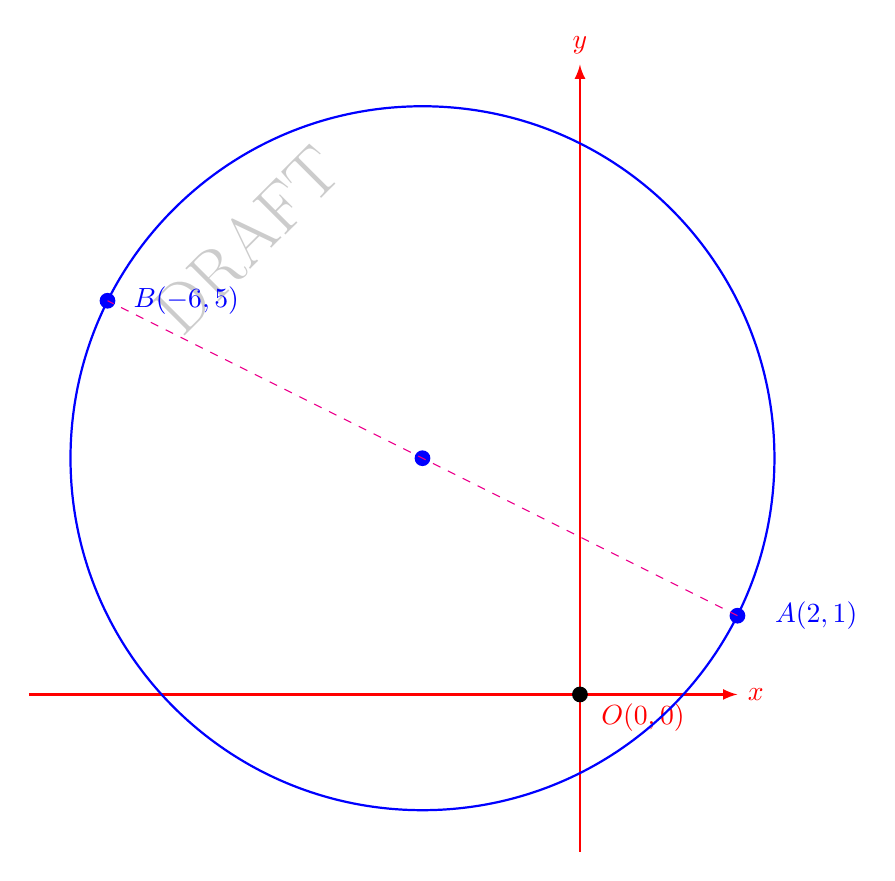
\begin{tikzpicture}[transform shape,scale=1]
		\draw [-latex,thick,red](-7,0) -- (2,0) node[right] {$x$} coordinate(x axis);
		\draw [-latex,thick,red](0,-2) -- (0,8) node[above] {$y$} coordinate(y axis);
		\fill[black] (0,0) circle (1 mm);
		\node at (0.8,-0.3) {$\textcolor{red}{O(0,0)}$};	
		\draw[thick,blue] (-2,3) circle (4.47);
		\fill[blue] (-2,3) circle (1 mm);
		\fill[blue] (-6,5 ) circle (1 mm);
		\fill[blue] (2,1) circle (1 mm);
		\node at (3,1) {$\textcolor{blue}{A(2,1)}$};
		\node at (-5,5) {$\textcolor{blue}{B(-6,5)}$};
		\draw[magenta,dashed](2,1)--(-6,5);
	\end{tikzpicture}\\
\\
		\textcolor{blue}{[বরিশাল বোর্ড-২০২২]}\\
	$A\left(\frac{5}{2},0\right)$ এবং  $B\left(0,\frac{3}{2}\right)$ বিন্দুদ্বয়ের সংযোগ রেখাংশকে ব্যাস ধরে অঙ্কিত বৃত্তের সমীকরণ নির্ণয় কর । \\
	\\
	\\
	$(x_1,y_1)=\left(\frac{5}{2},0\right)$ $(x_2,y_2)=\left(0,\frac{3}{2}\right)$\\
	\\
	\begin{align*}
		(x-x_1)(x-x_2)+(y-y_1)(y-y_2)&=0\\
		\\
		\left(x-\frac{5}{2}\right)(x-0)+(y-0)\left(y-\frac{3}{2}\right)&=0\\
		\\
2x^2+2y^2-5x-3y&=0	
\end{align*}
		\begin{tikzpicture}[transform shape,scale=1]
		\draw [-latex,thick,red](-6,0) -- (6,0) node[right] {$x$} coordinate(x axis);
		\draw [-latex,thick,red](0,-6) -- (0,6) node[above] {$y$} coordinate(y axis);
		\fill[black] (0,0) circle (1 mm);
		\node at (0.8,-0.3) {$\textcolor{red}{O(0,0)}$};	
		\draw[thick,blue] (1.25,0.75) circle (1.45);
		\fill[blue] (1.25,0.75 ) circle (1 mm);
		\fill[blue] (2.5,0 ) circle (1 mm);
		\fill[blue] (0,1.5) circle (1 mm);
		\draw[magenta,dashed](2.5,0)--(0,1.5);
	\end{tikzpicture}\\
	\\
\textcolor{blue}{$(x_1,y_1)$ ও $(x_2,y_2)$ বিন্দু দুইটির সংযোগ রেখাংশকে ব্যাস ধরে অঙ্কিত বৃত্তের সমীকরণ }	\\
	\\ 
	$D(x,y)$ বৃত্তের উপরস্থ যেকোনো বিন্দু \\
	\\
	অর্ধ বৃত্তস্থ কোণ $\angle ADB$ এক সমকোণ \\
	\\
	$AD$ এবং $BD$ পরস্পর লম্ব \\ 
	\\
$AD$ রেখার ঢাল ও $BD$ রেখার ঢালের গুনফল $=-1$\\ 
		\begin{tikzpicture}[transform shape,scale=1]
		\draw [-latex,thick,red](-2,0) -- (10,0) node[right] {$x$} coordinate(x axis);
		\draw [-latex,thick,red](0,-2) -- (0,10) node[above] {$y$} coordinate(y axis);
		\fill[black] (0,0) circle (1 mm);
		\node at (0.8,-0.3) {$\textcolor{red}{O(0,0)}$};	
		\draw[thick,blue] (5,5) circle (3);
		\fill[blue] (5,5) circle (1 mm);
		\node at (5,8.5) {$\textcolor{blue}{D(x,y)}$};
		\fill[blue] (5,8) circle (1 mm);
		\node at (1,5) {$\textcolor{blue}{A(x_1,y_1)}$};
		\fill[blue] (2,5) circle (1 mm);
		\node at (9,5) {$\textcolor{blue}{B(x_2,y_2)}$};
		\fill[blue] (8,5) circle (1 mm);
		\draw[red] (2,5)--(8,5);
		\draw[red] (2,5)--(5,8);
		\draw[red] (8,5)--(5,8);
	\end{tikzpicture}\\
	\\ 
	$AD$ রেখার ঢাল $=\frac{y-y_1}{x-x_1}$\\
	\\
	$BD$ রেখার ঢাল $=\frac{y-y_2}{x-x_2}$\\
	\\
	\begin{align*}
		\frac{y-y_1}{x-x_1}\times \frac{y-y_2}{x-x_2}&=-1\\
		\\
		\frac{(y-y_1)(y-y_2)}{(x-x_1)(x-x_2)}&=-1\\
		\\
		(y-y_1)(y-y_2)&=-(x-x_1)(x-x_2)\\
		\\
		(x-x_1)(x-x_2)+(y-y_1)(y-y_2)&=0
	\end{align*}
\end{document}